\subsection{Particle Swarm Optimization (PSO)}
PSO is an algorithm that simulates the sociological behavior of bird flocking. In the search space, we define a swarm $X$, which has many particles $x^p(t) \in \{x^1(t), x^2(t), \ldots, \gamma\}$ where $\gamma$ is a number of particles and $t$ is the $t$th iteration among $T$ total iterations. Each particle $x^p$ consists of many elements, $x^p_i$ where $i = 1,2,3, \ldots, \kappa$, with $\kappa$ is the dimension of a particle.

Firstly, the particles of the swarm are initialized and evaluated by a predefined fitness function. The objective of the PSO is to minimize these fitness function values. In order to move the particle in the search space, a velocity $v^p_j(t)$ is defined. It is the flight speed of the $j$th element of the $p$th particle at the $t$th iteration. Additionally, $x^p_j(t)$ is the current position of that element. The velocity and current position is then calculated by the following formulae:
\begin{equation}
v_{j}^{p}(t) = 2 \cdot rand() \cdot (pbest_{j}^{p} - x_{j}^{p}(t-1))
+ 2 \cdot rand() \cdot (gbest_{j} - x_{j}^{p}(t-1))
\end{equation}

\begin{equation}
x^p_j(t) = x^p_j(t - 1) + v^p_j(t)
\end{equation}

Another improved version of PSO which is introduced in \cite{eberhart2000comparing}, added two factors: the constriction and inertia which change the velocity calculation to:

\begin{equation}
v_{j}^{p}(t) = k \cdot \{w \cdot v^p_j(t-1) + \varphi_1 \cdot rand() \cdot (pbest_{j}^{p} - x_{j}^{p}(t-1))
+ \varphi_2 \cdot rand() \cdot (gbest_{j} - x_{j}^{p}(t-1)) \}
\end{equation}

where $k$ is the constriction factor and $w$ is the inertia factor, $\varphi_1$ and $\varphi_2$ are constants.

Even with the improved version of PSO, when the particle coincides with the global best position, the particle will move away from this point if the two factors above are different from zero. Furthermore, the particles will stop moving when their velocities are close to zero and they catch up with the global best position. This phenomena is called $stagination$ \cite{eberhart1998comparison}. To overcome this phenomena, the mutation process of GA has been added to PSO to form up a Hybrid PSO with Mutation (HPSOM). We will discuss this mutation process among with the Wavelet Mutation in the next section.

\subsection{Hybrid PSO with Wavelet Mutation}
The initial version of PSO with mutation process works as follows: a random particle is selected to be moved to another position in the search space by using mutation under the following operation:
\begin{equation}
mut(x_j) = x_j - \omega, r < 0
\end{equation}
\begin{equation}
mut(x_j) = x_j + \omega, r \geq 0
\end{equation}
where $x_j$ is a randomly chosen element of the particle above, $\omega$ is randomly generated in the range of $[0, 0.1 x (para^j_{max} - para^j_{min})]$, $r$ is a random number between +1 and -1, $para^j_{max}$ and $para^j_{min}$ are the upper and lower bounds of each particle element. Therefore, we can see that $\omega$ represents $1/10$ of the search space.

This version of PSO can overcome the $stagination$ phenomena. However, it can easily be seen that the mutating space is fixed by $\omega$. It is not always the best strategy for using the same size mutation space all the time. Therefore, in \cite{ling2008hybrid}, the author proposed an improvement method to dynamically adjust the mutating size $\omega$ based on the wavelet theory as follows.

\subsubsection{Hybrid PSO with Wavelet Mutation}
\
Each particle element has a chance to mutate which is controlled by a probability of mutation $p_m \in [0, 1]$. For each element, we generate a random number between 0 and 1 $r$, if $r \leq p_m$, the mutation will take place on that element. In details, let $x^p(t) = [x^p_1(t), x^p_2(t), \ldots, x^p_k(t)]$ be the current selected particle, with $x^p_j(t)$ is its randomly chosen element, $x^p_j(t) \in [param^j_{min}, param^j_{min}]$. After the mutation process, the resulting particle is $\bar{x}^p(t)$

\[ \bar{x}^p(t) = \left\{ \begin{array}{ll}
         x^p_j(t) + \sigma \times (para^j_{max} - x^p_j(t)) & \mbox{if $\sigma > 0$} \\
        x^p_j(t) + \sigma \times (x^p_j(t) - para^j_{min}) & \mbox{if $\sigma \leq 0$}.\end{array} \right. \] 

where $j \in 1,2,3, \ldots k$ is the dimension of the particle and:
\begin{equation}
	\sigma = \frac{1}{\sqrt{a}}\psi(\frac{\varphi}{a})
\end{equation}

where $\psi(x)$ is a wavelet - a continuous time function (see Figure \ref{fig:fig1}) represents a certain seismic signal that satisfies two properties:

\begin{equation}
	\int_{-\infty}^{+\infty}\psi(x)dx = 0
\end{equation}

and

\begin{equation}
	\int_{-\infty}^{+\infty}|\psi(x)|^2dx < 0
\end{equation}

\begin{figure} [H]
\centering
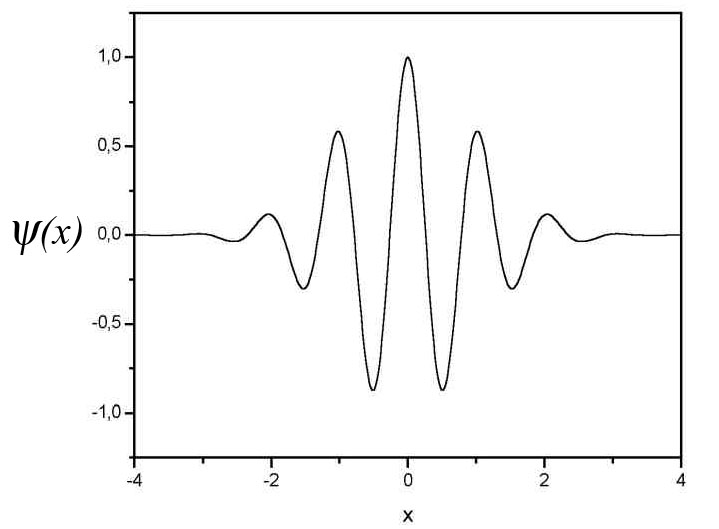
\includegraphics[width=60.72mm]{resources/morlet1}
\caption{The original form of the Morlet wavelet}\label{fig:fig1}
\end{figure}

In this paper, we adapt this approach (HPSOWM) and transform the real-valued particles into binary-based ones. This will be discussed in the next section.